\doublespacing
\setlength{\parindent}{1cm}

\begin{flushleft}
  \textbf{Design of an End to End Raga Data Pipeline}
\end{flushleft}

For this thesis, I had to think of a way to get a dataset of images that I can then use for training a convolutional neural network architecture. In order to go about this process, I decided to first understand how I will look at getting audio files in which I know the raga associated with each file. I will then convert each audio file into a chromagram with a short term Fourier transform in order to get spectral information as well as differences in pitch over the duration of the audio file. In order to get multiple chromagrams for each audio file, I decided to generate a chromagram for each minute of the audio file's duration. To make this possible, I had to use an advanced I\/O feature in Librosa known as blockwise reading. Since Librosa did not have blockwise reading on its own, I had to make use of another library in tandem with Librosa for making this possible. The name of this second library is known as PySoundFile which is a Python wrapper for SoundFile which makes blockwise-reading possible as well as a functionality for metadata information regarding any input audio file as long as it in a .wav format. This premise presented a challenge for me as it required a conversion from a compressed .mp3 format of medium quality into .wav to input files as arguments into SoundFile's functional interface.

\begin{flushleft}
  \textbf{Converting from MP3 to WAV}
\end{flushleft}

Since MP3 files are a compressed, digital format of audio data based on the bit rate measured in kilobits per second [ref], I first decided to look into those values surrounding the mp3 quality from my initial dataset of mp3 files. Since the dataset is based on medium-quality mp3 files, I deduced that the bit rate, x, will be a range bounded between $ (128 < x < 320) $ kbps depending on the extracted mp3 files from the dataset's architect. Since I do not have control over the variance in bit rates nor time to generate a uniform dataset of mp3 files, I decided to go straight into the conversion of the mp3 format to the wav format. In order to do this, I made use of a Python module known as scikit-sound. Scikit-sound [ref] is a very useful utility as it makes it possible to read compressed audio file formats and encode them into wav format by making use of a third party utility known as FFMPEG. FFMPEG has a sampling algorithm to scale various audio formats based on the type of audio conversion that needs to be done. For the case of scaling from mp3 to wav in which the file size is much greater, FFMPEG samples at a standard sampling rate based on a default encoding from mp3 to wav. The encoding is not readily observable by the end user. FFMPEG is considered as the engine within scikit-sound's Sound class. From the software point of view, a simple instantiation of the Sound class with the input being the mp3 file will automatically read a wav file of the same file name while disregarding the .mp3 extension. Fortunately, FFMPEG is available across many operating systems and so I was able to install it using the Homebrew package manager within my Macbook. The uniform sampling rate from FFMPEG becomes a huge convenience when going into block reading which will be discussed more specifically in the next section.

\begin{lstlisting}
  # An instance of Scikit-Sound's Sound Class
  # Python 3.6+
  from sksound.sounds import Sound
  import os

  fileList = os.listdir("/path to raga audio files in mp3 format")
  # dictionary to store each instantiated response
  fileDict = {}
  # iterating through every file
  for file in fileList:
    fileDict[file] = Sound(f"path/{file}")
\end{lstlisting}

Each wav file will be in the same directory as the path which contains the mp3 files. To alleviate this challenge, I created a directory structure as follows:

\begin{figure}
  \caption{Directory Structure for Audio Files}
  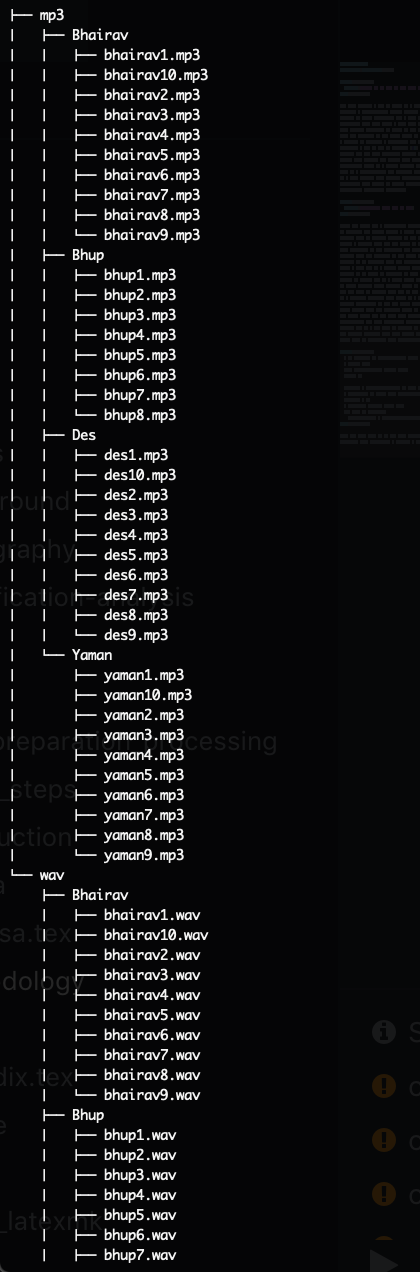
\includegraphics{audio-directory.png}
  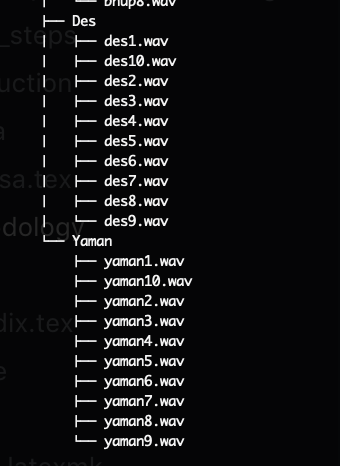
\includegraphics{audio-directory2.png}
\end{figure}

Once the wav files finished generating for each specific raag, I ran the following bash commands in my Terminal to move all the wav files into the wav directory.

\begin{lstlisting}
  cd data/Hindustani/mp3/Bhairav && mv *.wav ../../wav/Bhairav
  cd data/Hindustani/mp3/Bhup && mv *.wav ../../wav/Bhup
  cd data/Hindustani/mp3/Des && mv *.wav ../../wav/Des
  cd data/Hindustani/mp3/Yaman && mv *.wav ../../wav/Yaman
\end{lstlisting}

I also want to note that in order to perform proper version controlling of all my code commits, I tracked all mp3 and wav files using git-lfs so they would be known to Git and my GitHub repository as large files and will therefore be written to GitHub upon pushing commits with a higher file writing rate than that of normally pushed files.

\begin{flushleft}
  \textbf{Block-Wise Reading with PySoundFile}
\end{flushleft}

As mentioned before, I wanted to read the audio files as blocks of a certain size in order to generate stft-chromagrams for each minute in every audio file. To calculate the block size, b, I used the following equation in which sr refers to the sampling rate per second and n refers to the number of seconds:

$$ b = sr * n $$

To get the specific sampling rate which FFMPEG used for sampling, I used an attribute of PySoundFile.

\begin{lstlisting}
  # importing PySoundFile
  import soundfile as sf
  import os
  bhairavList = os.listdir("data/Hindustani/wav/Bhairav")
  for file in bhairavList:
    rate = sf.info(f"data/Hindustani/wav/Bhairav/{file}").samplerate
    print(rate)
\end{lstlisting}

The sampling rate that FFMPEG used for converting from mp3 to wav for the audio files corresponding to each raga is 44100 Hz. This means that in order to get a chromagram for each minute in the audio file, n would have to be equal to 60 since there are 60 seconds in a minute.

My uniform blocksize computes to:

$$ b = 44100 * 60 = 2646000 $$

After getting this value, reading in audio files into Librosa in tandem with PySoundFile's functionality became a very trivial matter.

\begin{lstlisting}
import numpy as np
# importing soundfile and librosa
!pip install pysoundfile
import soundfile as sf
from librosa.feature import chroma_stft
from librosa.display import specshow
import matplotlib.pyplot as plt
# Bhairav Block Wise Reading

## Bhairav 1

block_gen = sf.blocks('data/Hindustani/wav/Bhairav/bhairav1.wav', blocksize=2646000)
rate = sf.info("data/Hindustani/wav/Bhairav/bhairav1.wav").samplerate
info = sf.info("data/Hindustani/wav/Bhairav/bhairav1.wav")
print(info)
chromas = []

for bl in block_gen:
    y = np.mean(bl, axis=1)
    chromas.append(chroma_stft(y, sr=rate))

len(chromas)
for j, chroma in enumerate(chromas):
    specshow(chroma, x_axis="time", y_axis="chroma", vmin=0, vmax=1)
    plt.title(f"Chromagram of Bhairav1_{j}")
    plt.savefig(f"data/chroma_files/bhairav-chromas/bhairav1/bhairav1_{j}.png")
\end{lstlisting}

The above script allowed me to automate the generation of stft-chromagrams for every one minute block in the first audio recording of raga Bhairav. After thinking about the iterative process, I managed to build a more powerful automation script that would be able to generate chromagrams for every block for every audio file for a specific raga.  An example of this process is shown below to generate stft-chromagrams for all the audio files of the dataset I used for raga, Bhup.

\begin{lstlisting}
import os
import numpy as np
import soundfile as sf
from librosa.feature import chroma_stft
from librosa.display import specshow
import matplotlib.pyplot as plt

bhup_files = os.listdir("data/Hindustani/wav/Bhup")
print(bhup_files)

# Generating directories to denote each bhup audio file an iterative path

for h,i in enumerate(bhup_files):
    os.system(f"mkdir data/chroma_files/bhup-chromas/bhup{h+1}")

# Creating an empty dictionary to store

chroma_dict = {}

for j in range(len(bhup_files)):

    # building blocks for each file pertaining to the Bhup raga

    rate = sf.info(f"data/Hindustani/wav/Bhup/bhup{j+1}.wav").samplerate
    block_gen = sf.blocks(f"data/Hindustani/wav/Bhup/bhup{j+1}.wav", blocksize=rate*60)
    chroma_dict[f"bhup{j+1}"] = []

    # Computing the chroma_stft for every block in each Bhup audio file

    for bl in block_gen:
        y = np.mean(bl, axis=1)
        chroma_dict[f"bhup{j+1}"].append(chroma_stft(y, sr=rate))

    # Visualizing and saving the stft-chromagram for every block for every Bhup audio file
    # naming convention: bhup[file enumeration]_[block number]

    for k, chroma in enumerate(chroma_dict[f"bhup{j+1}"]):
        specshow(chroma, x_axis="time", y_axis="chroma", vmin=0, vmax=1)
        plt.title(f"Chromagram of Bhup{j+1}_{k+1}")
        plt.savefig(f"data/chroma_files/bhup-chromas/bhup{j+1}/bhup{j+1}_{k+1}.png")
\end{lstlisting}

The figure below illustrates the file structure for the generated chromagrams as png files.

\begin{figure}
  \caption{File Structure for Stored Bhup and Bhairav STFT-Chromagram Images}
  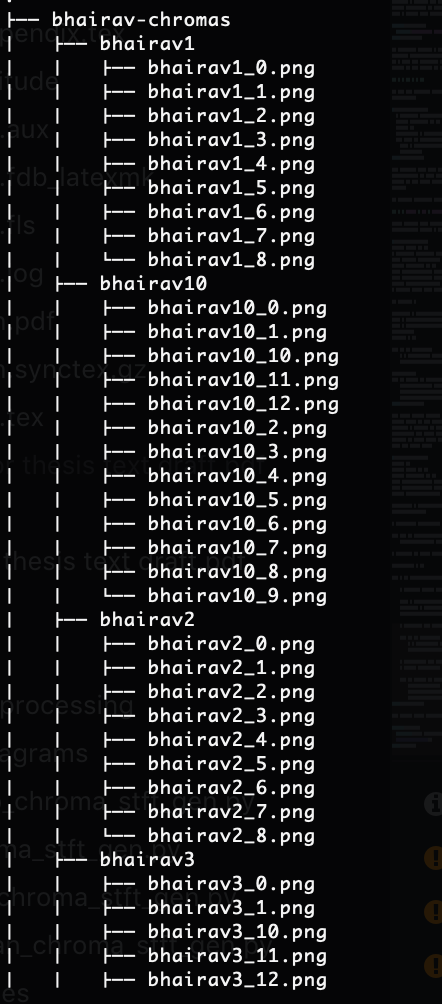
\includegraphics{bhairav-chroma-tree.png}
  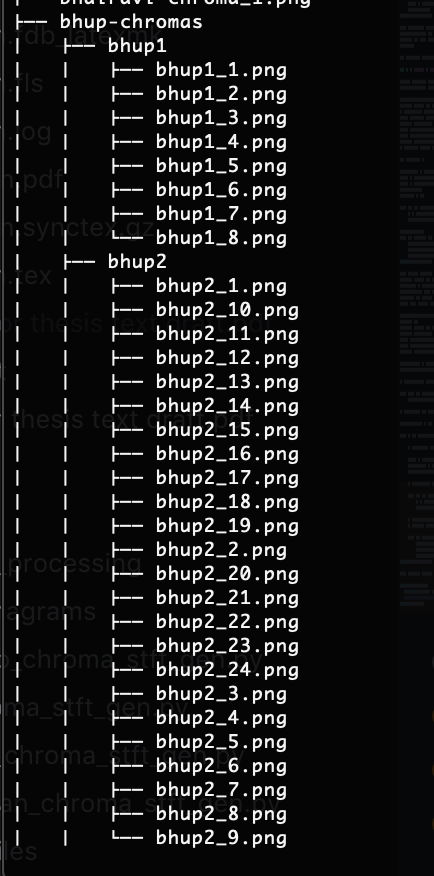
\includegraphics{bhup-chroma-tree.png}
\end{figure}

\begin{flushleft}
  \textbf{Data Preparation for CNN Training}
\end{flushleft}

In order to have the images ready for a machine learning experiment with a convolutional neural network, I first needed to generate a csv file of labels corresponding to the raga of each recording. Since I had an original file structure comprising of all the images of all the ragas, building up labels for all the files became very trivial and the ragas were all in
alphabetical order. The script below shows the process I used in pandas to build the miml\_labels\_2 csv file.

\begin{lstlisting}
import pandas as pd
import os

# Empty dictionary

columnDict = {}

# Getting all image files in one Python list

fileList = os.listdir("data")
print(len(fileList))

columnDict['file_name'] = fileList

print(columnDict)

# Empty list to store labels

labels = []

# Range values calculated beforehand

for i in range(202):
  labels.append("bhairav")

for i in range(183):
  labels.append("bhup")

for i in range(137):
  labels.append("des")

for i in range(258):
  labels.append("yaman")

print(len(labels))

# Generating second column to store labels

columnDict['raga'] = labels

# Converting from a dictionary to a Pandas DataFrame

df = pd.DataFrame.from_dict(columnDict)

# Saving DataFrame as a Comma Separated Value (csv) file

df.to_csv("csv/miml_labels_2.csv")

\end{lstlisting}

\begin{flushleft}
  \textbf{CNN Preprocessing and Training with Tensorflow 2.0 and Keras on Google Colab}
\end{flushleft}

Now that I had my CSV file and image data, I moved over from my local environment to Google Colaboratory in order to make use of a free tier graphics processing unit (GPU) optimized for neural network training with ease offered by the Google Compute Engine (GCE) with a memory allocation of 12 GB RAM.
\par
In order to make this transition simple, I created another GitHub repository which contains 780 stft-chromagram images as well as the csv file pertaining to labels that correspond in order of the files. Since Git and several popular Python modules are already pre-installed in Google Colaboratory's Jupyter notebook interface, I easily cloned my repository into Colaboratory and changed the notebook's base directory to the repository's directory for ease of file reading. The next step is to build a convolutional neural network architecture.
\par
The resolution for each stft-chromagram is 432 X 288 pixels therefore I decided to add in more than just two convolutional layers in the architecture. The architecture I decided to use is 2 convolutional layers, a max pooling layer, another set of two convolutional layers, and then another max pooling layer and then a connection from the second max pooling layer to the hidden layer of 512 neurons and then a final connection from the hidden layer to an output layer of 4 neurons where the classification decision is made by the softmax activation function. All other layers have a rectified linear unit activation function. This architecture is shown in Tensorflow's 2.0 Keras module below.

\begin{lstlisting}
classifier = Sequential()
classifier.add(Conv2D(32, (3, 3), padding='same', input_shape = (432, 288, 3), activation = 'relu'))
classifier.add(Conv2D(32, (3, 3), activation = 'relu'))
classifier.add(MaxPooling2D(pool_size = (2, 2)))
classifier.add(Dropout(rate=1-0.25))
classifier.add(Conv2D(64,(3,3), padding="same", activation="relu"))
classifier.add(Conv2D(64, (3,3), activation="relu"))
classifier.add(MaxPooling2D(pool_size=(2,2)))
classifier.add(Dropout(rate=1-0.25))
classifier.add(Flatten())
classifier.add(Dense(units = 512, activation = 'relu'))
classifier.add(Dropout(rate=1-0.5))
classifier.add(Dense(units = 4, activation = 'softmax'))
classifier.compile(optimizer = 'adam', loss = 'categorical_crossentropy', metrics = ['accuracy'])
\end{lstlisting}
